\chapter*{¿Dónde debería un piloto iniciar su aterrizaje?}
\begin{wrapfigure}{l}{0.5\textwidth}
	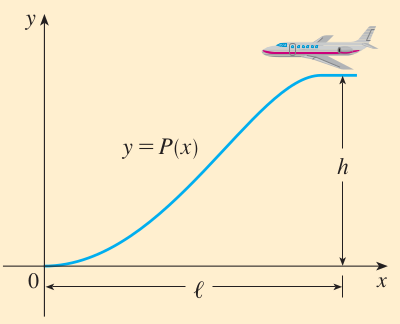
\includegraphics[height = 0.25\textheight]{recursos/Captura desde 2024-09-21 16-53-03.png}
\end{wrapfigure}
\noindent
En la figura se muestra una trayectoria de aproximación para el aterrizaje de un avión, que satisface las condiciones siguientes:

\begin{enumerate}[label=\Roman*)]
	\item La altura del crucero es $h$ cuando se inicia el descenso a una distancia $l$ del punto de contacto con la pista en el origen.
	\item El piloto debe mantener una rapidez horizontal constante $v$ a todo lo largo del descenso.
	\item El valor absoluto de la aceleración vertical no debe sobrepasar una constante $k$ (la cual es mucho menor que la aceleración debida a la gravedad).
\end{enumerate}